\documentclass[
	%article, % se for trabalho academico, isso tem que ser comentado
	12pt,
	oneside,
	a4paper,
	chapter=TITLE,
	section=TITLE,
	english,
	brazil,
	sumario=tradicional
]{abntex2}


\usepackage[utf8]{inputenc}
\usepackage{array}
\usepackage{geometry}
\usepackage{multirow}
\usepackage{graphicx}
\usepackage{estrutura}
\usepackage{float}
\usepackage{pgfplots}
\usepackage{xcolor}
\usepackage{listings}


% podem dar problema, e terá que ajustar o espaçamento manualmente
%\usepackage{fontspec} % Pacote para carregar fontes do sistema
%\setmainfont{Arial} % Define a fonte principal como Arial


% semelhante a arial, gera menos erro, mas ainda gera erros
%\usepackage{helvet} % Carrega a fonte Helvetica
%\renewcommand{\familydefault}{\sfdefault} % Define a fonte sem serifa como padrão



% ---
% Dados do documento
% ---



%\tipotrabalho{Artigo}


% --- 
\titulo{Relatório Técnico - Processamento Paralelo em Cluster Ubuntu}
\autor{Felipe William Galdino da Silva, \\ João Carlos G. Iannuzzi, \\ Reyner C. Silva Alegria }
\local{Itacoatiara - Am}
%\orientador{James Roberto Chaves de Araújo}
%\data{2025} % imprime o ano corrente no campo data
\data{\the\year}
%\instituicao{Universidade Federal do Amazonas}
%\tipotrabalho{Relatório Técnico}
\preambulo{Trabalho apresentado ao professor Antonio Alberto Sena dos Santos do Instituto de Ciências Exatas e Tecnologia da Universidade Federal do Amazonas, como atividade prática para a obtenção de nota na disciplina de Sistemas Distribuídos.}
% ---


%\date{}
%\definirautores

\makeindex

\setlrmarginsandblock{3cm}{3cm}{*}
\setulmarginsandblock{3cm}{3cm}{*}
\checkandfixthelayout
\setlength{\parindent}{1.3cm}
\setlength{\parskip}{0.2cm}
\setlength{\ABNTEXcitacaorecuo}{1.8cm}
%\SingleSpacing
\OnehalfSpacing

% ----
% Início do documento
% ----

\begin{document}

    %\begin{tikzpicture}[remember picture, overlay]
      %  \tikzset{inner sep=0pt, outer sep=0pt}
     %   \node at (current page.center)
       % {\includegraphics[height=\paperheight]%{imagens/PIBIC.pdf}};
  %  \end{tikzpicture}
	
	% Seleciona o idioma do documento
	\selectlanguage{brazil}
	
	% Retira espaço extra obsoleto entre as frases.
	\frenchspacing 
	
	% ----------------------------------------------------------
	% ELEMENTOS PRÉ-TEXTUAIS
	% ----------------------------------------------------------
	
	% Se desejar escrever o artigo em duas colunas, descomente a linha abaixo
	% e a linha com o texto "FIM DE ARTIGO EM DUAS COLUNAS".
	% \twocolumn[    		% INICIO DE ARTIGO EM DUAS COLUNAS
    
	% título
	%\maketitle
	\begin{capa}
		\pdfbookmark[0]{Capa}{capa}
		\thispagestyle{empty}
		\centering
		\begin{center}
			
			\begin{comment} % caso queira fazer manualmente
			
				\begin{minipage}{1\linewidth}
					\centering
					\begin{tabular}{cp{20.89em}c}
						\begin{tabular}{c}
							\\
							
\includegraphics[width=1.9cm]{imagens/marca_ufam_vetor_positivo.png}
						\end{tabular}
						&
						\begin{tabular}{c}
							\\
							{\large \imprimirinstituicao} \\
							{\large Instituto de Ciências Exatas e Tecnologia} \\
							{\large Bacharelado em Engenharia de Software} \\
							%{\large Engenharia de Controle e Automação}
						\end{tabular}
						&
						\begin{tabular}{c}
							\\
							
\includegraphics[width=3.1cm]{imagens/ICET.png}
						\end{tabular}
					\end{tabular}
				\end{minipage}
			
			\end{comment}
			
			\begin{tikzpicture}[remember picture, overlay]
				\tikzset{inner sep=0pt, outer sep=0pt}
				\node at (current page.center)
				{
\includegraphics[height=\paperheight]{imagens/Cabeçalho.pdf}};
			\end{tikzpicture}
			
			
			\centering
			\vspace*{1cm}
			{\ABNTEXsectionfont\large\imprimirautor}
			\vspace*{\fill}
			
			{\ABNTEXsectionfont\bfseries \large \imprimirtitulo}
			\vspace*{\fill}
			
			{\large\imprimirtipotrabalho}
			\vspace*{\fill}
			
			\begin{tabular}{c}
				{\large\imprimirlocal} \\
				{\large\imprimirdata}
			\end{tabular}
			%\par
			\vspace*{1cm}
		\end{center}
	\end{capa}
	
	\imprimirfolhaderosto
	
	
	\tableofcontents
	\newpage
	% resumo em português
% \begin{resumo}
		
% %Este trabalho apresenta uma análise comparativa de desempenho entre duas bibliotecas de processamento paralelo, Pthreads e OpenMP, aplicadas ao problema de busca linear em vetores de grande dimensão. Foram implementadas versões sequenciais e paralelas em linguagem C, variando-se o tamanho da entrada (até 100 milhões de elementos) e o número de threads (até 16). Os resultados experimentais, avaliados através das métricas de Speedup e Eficiência, demonstraram que a abordagem com OpenMP obteve ganhos de desempenho significativos e escalabilidade consistente. Em contrapartida, a implementação manual com Pthreads sofreu degradação de performance (slowdown) devido à alta contenção de recursos na sincronização, evidenciando a importância da escolha correta das primitivas de controle de concorrência.
		
% 		\vspace{\onelineskip}
		
%         % todas em letras minúsculas, separadas por ponto e vírgula (;)
%         %\textbf{Palavras-chave}: Processamento Paralelo, OpenMP, Pthreads, Busca Linear, Speedup.
		
% \end{resumo}

\textual
   
\section{Introdução}
%\addcontentsline{toc}{section}{Introdução}

O presente trabalho tem como propósito a configuração e experimentação de um ambiente de computação distribuída, utilizando um \textit{cluster} composto por quatro máquinas virtuais orquestradas sob o paradigma de processamento paralelo com MPI (\textit{Message Passing Interface}). O problema central explorado é a estimativa do valor de $\pi$ (Pi) por meio do Método de Monte Carlo — uma técnica probabilística que simula o lançamento de um bilhão de pontos aleatórios em um espaço bidimensional, utilizando a proporção dos pontos que caem dentro de um círculo inscrito em um quadrado para aproximar o valor da constante matemática. Embora conceitualmente simples, o volume massivo de iterações exigido torna a execução sequencial em uma única máquina computacionalmente custosa, evidenciando a necessidade de distribuição da carga de trabalho. Nesse contexto, a atividade propõe a divisão igualitária das iterações entre um nó mestre e três nós trabalhadores (\textit{workers}), permitindo que o processamento ocorra em paralelo e, ao final, os resultados parciais sejam consolidados via \textit{MPI Reduce}. O experimento visa não apenas verificar a aceleração (\textit{speedup}) obtida com o uso do \textit{cluster} em relação à execução serial, mas também aprofundar a compreensão sobre os três pilares fundamentais dos sistemas distribuídos: comunicação entre nós via rede e SSH, sincronização das tarefas paralelas através do MPI, e escalabilidade do sistema frente ao aumento do número de processos.

\section{Metodologia}

A metodologia desta atividade foi estruturada em cinco fases sequenciais, cada uma construindo sobre a anterior para garantir um ambiente distribuído funcional e reproduzível. A seguir, cada fase é detalhada com suas justificativas técnicas.

\subsection{Provisionamento das Máquinas Virtuais}

O primeiro passo consistiu na criação de quatro máquinas virtuais (VMs) utilizando o hipervisor \textit{VirtualBox}. A escolha por virtualização, em vez de máquinas físicas dedicadas, se justifica pela viabilidade prática do ambiente acadêmico: VMs permitem simular um \textit{cluster} real em um único computador \textit{host}, com custo zero de hardware adicional e total controle sobre a configuração de rede.

Foram criadas quatro VMs com as especificações descritas na Tabela \ref{tab:especificacoes}:

\begin{table}[H]
    \centering
    \caption{Especificações das máquinas virtuais}
    \begin{tabular}{|l|l|l|}
        \hline

        \rowcolor{gray!25} 
        \textbf{Máquina} & \textbf{RAM} & \textbf{CPUs} \\ 
        \hline
        
        % Linhas de Dados
        master & 1GB & 2 \\ 
        \hline
        node1 & 1 GB & 2  \\ 
        \hline
        node2 & 1GB & 2  \\ 
        \hline
        node3 & 1 GB & 2  \\ 
        \hline
    \end{tabular}
    
    \label{tab:especificacoes}
\end{table}

A alocação de apenas 1 GB de RAM e 2 CPUs por VM foi uma decisão deliberada para não sobrecarregar o computador \textit{host}, já que quatro VMs rodam simultaneamente. O desempenho individual de cada nó é secundário neste experimento — o que se avalia é o ganho coletivo do \textit{cluster}.

O sistema operacional escolhido foi o \textit{Ubuntu Server 22.04 LTS}. A versão \textit{Server} (sem interface gráfica) foi preferida à versão \textit{Desktop} pois consome significativamente menos memória RAM e processamento, recursos escassos no cenário de múltiplas VMs simultâneas. A designação LTS (\textit{Long Term Support}) garante estabilidade e suporte de atualizações de segurança por cinco anos, sendo a escolha padrão da indústria para servidores em produção.

\begin{figure}[h]
  \centering
  
    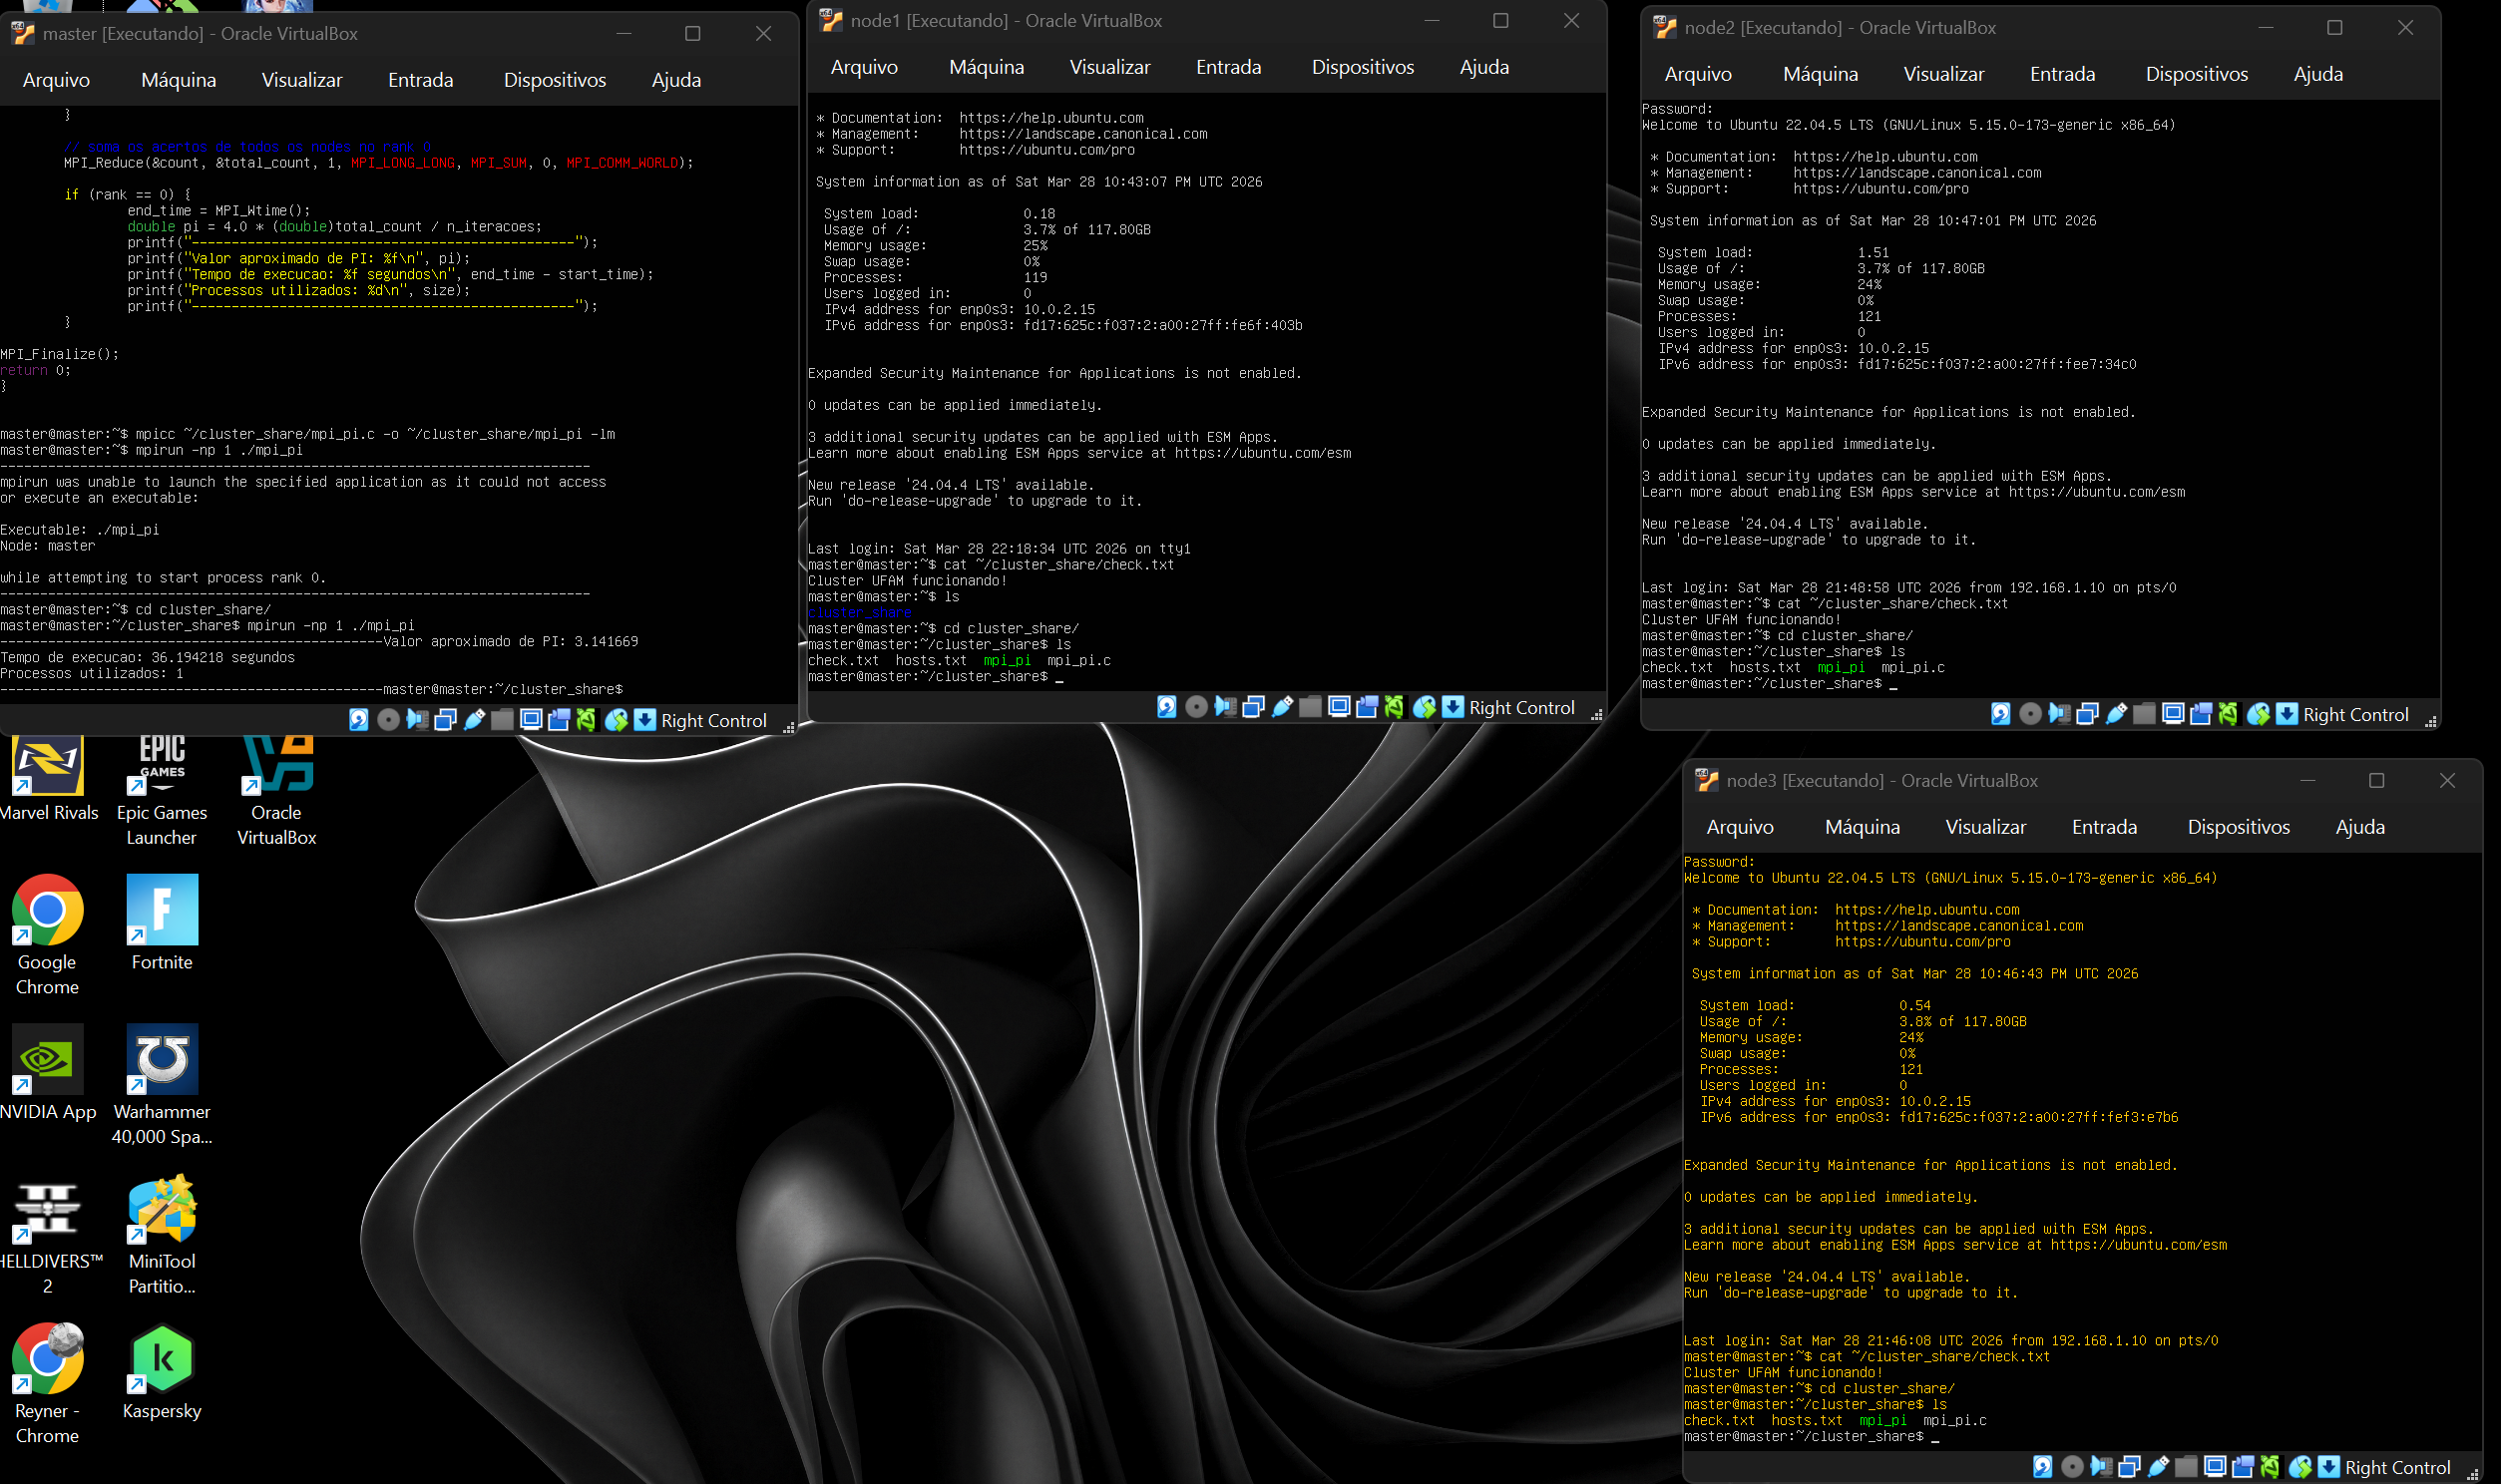
\includegraphics[width=0.85\textwidth]{imagens/VMS.png}
    \caption{Demonstração do hipervisor mostrando as 4 VMs criadas.}
  \label{fig:nfsserver}
\end{figure}

\subsection{Configuração de Rede e Identificação dos Nós}

Para que as máquinas de um cluster possam se comunicar de forma
confiável, cada VM foi configurada com dois adaptadores de
rede no VirtualBox, cada um com uma função distinta e complementar.
 
O primeiro adaptador opera em modo \textbf{NAT}
(\textit{Network Address Translation}). Neste modo, o \textit{VirtualBox}
funciona como um roteador intermediário: a VM acessa a internet
através do IP do computador hospedeiro, sem precisar de um IP
público próprio. Este adaptador foi necessário exclusivamente para
permitir o acesso à internet durante a instalação de pacotes via
\texttt{apt} (compilador, MPI, SSH). Ele não é utilizado para a
comunicação entre os nós do cluster.
 
O segundo adaptador opera em modo \textbf{Rede Interna}
(\textit{Internal Network}), com o nome de rede
\texttt{cluster\_net}. Este modo cria uma rede privada e isolada,
visível \emph{apenas} entre as VMs que compartilham o mesmo nome
de rede — completamente separada da rede física do hospedeiro.
É por esta interface que todo o tráfego do MPI e do SSH entre os
nós circula. O isolamento garante que não haja interferência de
outros dispositivos da rede física, tornando o ambiente do \textit{cluster}
controlado e previsível.

Com os adaptadores criados, foi necessário configurar um
IP fixo na interface do Adaptador~2 (\texttt{enp0s8})
em cada VM. IPs fixos são indispensáveis em um \textit{cluster}: se o
endereço de um nó mudasse a cada reinicialização (como ocorre
em DHCP), o \texttt{/etc/hosts} e os arquivos de configuração
do MPI ficariam desatualizados, quebrando a comunicação.
 
No Ubuntu Server 22.04, a configuração de rede é gerenciada pelo
\textit{Netplan}. O arquivo de configuração foi editado no nó
master e, posteriormente, adaptado em cada clone com o IP
correspondente:
 
\begin{lstlisting}[style=bash, caption={Edição do arquivo de configuração do Netplan no master.}]
sudo nano /etc/netplan/00-installer-config.yaml
\end{lstlisting}
 
\begin{lstlisting}[style=bash, caption={Conteúdo do arquivo Netplan configurando NAT (DHCP) e IP fixo na rede interna.}]
network:
  ethernets:
    enp0s3:          # Adaptador 1 - NAT (internet via DHCP)
      dhcp4: true
    enp0s8:          # Adaptador 2 - Rede Interna (IP fixo)
      addresses: [192.168.1.10/24]   # Ajustar por nó
  version: 2
\end{lstlisting}
 
A interface \texttt{enp0s3} corresponde ao Adaptador~1 (NAT) e
recebe seu IP automaticamente via DHCP do VirtualBox. Já a
\texttt{enp0s8} corresponde ao Adaptador~2 (Rede Interna) e
recebe um IP fixo atribuído manualmente, diferente para cada nó.
A notação \texttt{/24} define a máscara de sub-rede
\texttt{255.255.255.0}, o que significa que todos os nós do
cluster (na faixa \texttt{192.168.1.x}) pertencem à mesma rede
e conseguem se comunicar diretamente.
 
Após editar o arquivo, as configurações foram aplicadas com:
 
\begin{lstlisting}[style=bash, caption={Aplicação das configurações de rede.}]
sudo netplan apply
\end{lstlisting}
 
Os IPs fixos atribuídos a cada nó na rede interna estão
descritos na Tabela \ref{tab:mapeamento}.

\begin{table}[htb]
    \centering
   
    \begin{tabular}{|l|l|l|}
        \hline

        \rowcolor{gray!25} 
        \textbf{Máquina}  & \textbf{Endereço IP}  \\ 
        \hline
        
        % Linhas de Dados
        \texttt{master}   & \texttt{[192.168.1.10]} \\
        \hline
        \texttt{node1}    & \texttt{[192.168.1.11]} \\
        \hline
        \texttt{node2}    & \texttt{[192.168.1.12]} \\
        \hline
        \texttt{node3}    & \texttt{[192.168.1.13]} \\
        \hline
    \end{tabular}
    \caption{Mapeamento de nomes e endereços IP do cluster.}
    \label{tab:mapeamento}
\end{table}
 
Em seguida, o arquivo \texttt{/etc/hosts} foi editado em
\textbf{todas as quatro VMs}. Este arquivo é um mecanismo de
resolução de nomes local — ele instrui o sistema operacional a
associar um nome amigável (como \texttt{master} ou \texttt{node1})
a um endereço IP, sem depender de um servidor DNS externo. Isso é
essencial para o MPI, que localiza os nós do cluster pelos seus
nomes de \textit{host}.
 
\begin{lstlisting}[style=bash, caption={Edição do arquivo \texttt{/etc/hosts} em todos os nós.}]
sudo nano /etc/hosts
 
192.168.1.10 master
192.168.1.11 node1
192.168.1.12 node2
192.168.1.13 node3
\end{lstlisting}
 
\begin{figure}[h]
  \centering
  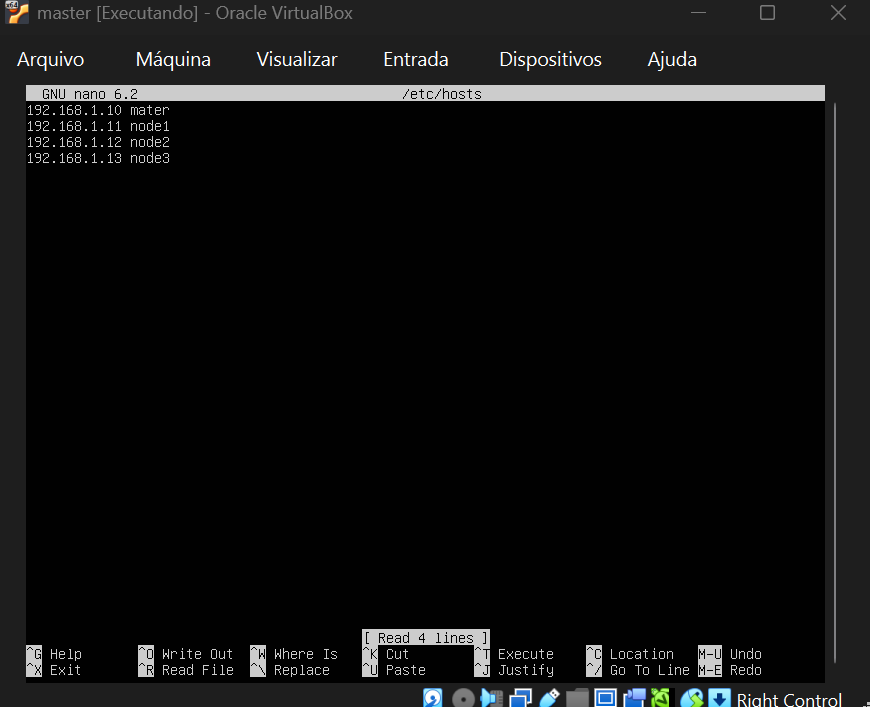
\includegraphics[width=0.75\textwidth]{imagens/etcHosts.png}
  \caption{Arquivo \texttt{/etc/hosts} configurado com os IPs e nomes do \textit{cluster}.}
  \label{fig:hosts}
\end{figure}


\subsection{Instalação das Dependências}

Esta fase foi executada em todas as quatro VMs, pois cada
nó do \textit{cluster} precisa ser capaz de compilar e executar o código MPI
de forma autônoma. Primeiramente, os repositórios do sistema foram
atualizados para garantir a instalação das versões mais recentes
dos pacotes:
 
\begin{lstlisting}[style=bash, caption={Atualização do sistema em todos os nós.}]
sudo apt update && sudo apt upgrade -y
\end{lstlisting}
 
Em seguida, foram instalados os três componentes essenciais:
 
\begin{lstlisting}[style=bash, caption={Instalação do compilador, servidor SSH e biblioteca MPI.}]
sudo apt install -y build-essential openssh-server openmpi-bin libopenmpi-dev nfs-kernel-server
\end{lstlisting}
 
Cada componente tem uma função específica e indispensável:
 
\begin{itemize}
 
  \item \textbf{\texttt{build-essential}} — Instala o compilador GCC
  e ferramentas essenciais de compilação em C (como \texttt{make} e
  \texttt{libc}). É necessário porque o algoritmo de Monte Carlo foi
  escrito em linguagem C, que precisa ser compilada antes de ser
  executada.
 
  \item \textbf{\texttt{openssh-server}} — Instala e ativa o servidor
  SSH (\textit{Secure Shell}) em cada nó. O MPI utiliza o SSH como
  canal de comunicação para iniciar processos remotamente nos nós
  \textit{workers} a partir do master. Sem o SSH ativo em todos os
  nós, o master não consegue distribuir e iniciar a execução do
  programa.
 
  \item \textbf{\texttt{openmpi-bin}} — Instala os binários do
  OpenMPI, incluindo o comando \texttt{mpirun}, responsável por
  lançar o programa paralelamente em múltiplos processos e nós.
  O OpenMPI é uma implementação de código aberto, madura
  e amplamente utilizada do padrão MPI, sendo a escolha natural
  para ambientes acadêmicos e de pesquisa.
 
  \item \textbf{\texttt{libopenmpi-dev}} — Instala os cabeçalhos
  (\textit{headers}) e bibliotecas de desenvolvimento do MPI. Esses
  arquivos são necessários em tempo de compilação: quando o compilador
  encontra a diretiva \texttt{\#include <mpi.h>} no código-fonte,
  é aqui que ele busca as definições das funções MPI. Sem este
  pacote, a compilação falharia.

  \item \textbf{\texttt{nfs-kernel-server}} — Instala o servidor NFS
  (\textit{Network File System}), o protocolo padrão do Linux para
  compartilhamento de diretórios entre máquinas em rede. No contexto
  deste cluster, o NFS permite que um diretório criado no nó master
  seja montado e acessado por todos os \textit{workers} como se fosse
  uma pasta local. Isso elimina a necessidade de copiar manualmente o
  executável compilado para cada nó via \texttt{scp}: basta compilar
  uma vez no master e todos os nós enxergam o arquivo automaticamente
  pelo diretório compartilhado.
 
\end{itemize}

\subsection{Configuração do SSH sem Senha}

Esta é uma das fases mais críticas para o funcionamento do \textit{cluster}.
O \texttt{mpirun}, ao ser executado no master, inicia processos nos
nós \textit{workers} automaticamente, sem intervenção humana. Se o
SSH solicitasse uma senha a cada conexão, o processo travaria.
 
A solução é a autenticação por par de chaves criptográficas
RSA. Neste mecanismo, o master gera duas chaves matematicamente
relacionadas: uma privada (guardada apenas no master) e
uma pública (distribuída para todos os nós). Quando o
master tenta se conectar a um nó, o nó verifica a assinatura com
a chave pública — se corresponder à chave privada, a autenticação
é aprovada sem necessidade de senha.
 
\paragraph{Passo 1 — Geração do par de chaves no master.}
 
\begin{lstlisting}[style=bash, caption={Geração do par de chaves RSA no nó master.}]
ssh-keygen -t rsa -N "" -f ~/.ssh/id_rsa
\end{lstlisting}
 
O parâmetro \texttt{-t rsa} especifica o algoritmo RSA para geração
das chaves. Ao ser solicitado um caminho e uma \textit{passphrase},
pressiona-se \texttt{Enter} em todas as opções para aceitar os
valores padrão e manter a chave sem senha adicional.
 
\begin{figure}[h]
  \centering
  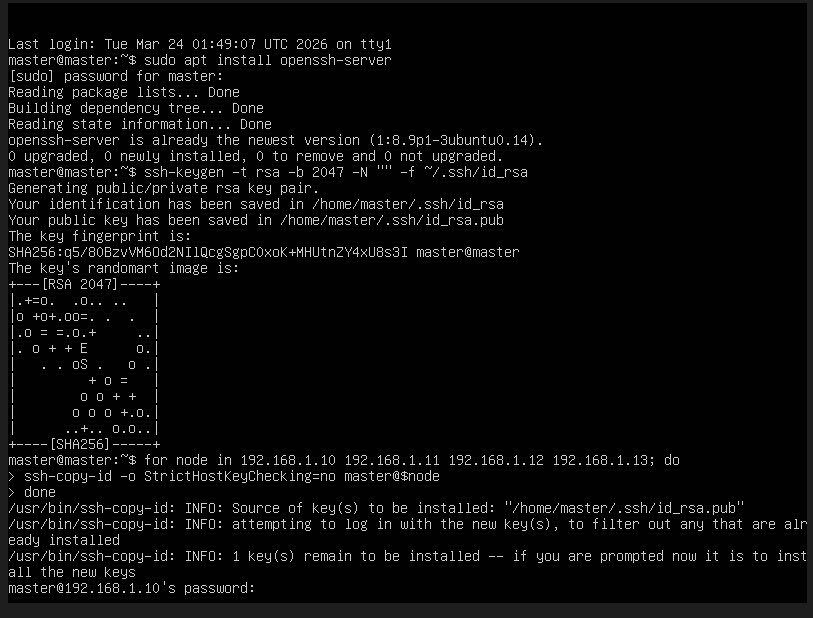
\includegraphics[width=0.75\textwidth]{imagens/geracaoChave.png}
  \caption{Geração do par de chaves RSA no nó master.}
  \label{fig:keygen}
\end{figure}
 
\paragraph{Passo 2 — Distribuição da chave pública para todos os nós.}
 
Ainda no nó master, a chave pública foi distribuída para todos os
nós do cluster — inclusive para o próprio master — por meio de um
laço \texttt{for} executado diretamente no terminal:

% \lstdefinestyle{bash}{language=bash, basicstyle=\ttfamily\small, keywordstyle=\color{blue}, commentstyle=\color{gray}, stringstyle=\color{red}, showstringspaces=false, columns=flexible}
 
\begin{lstlisting}[style=bash, caption={Laço executado no master para copiar a chave pública a todos os nós.}]
for maquina in master node1 node2 node3; do
    ssh-copy-id master@$maquina
done
\end{lstlisting}
 
O laço itera sobre cada nome de máquina definido no
\texttt{/etc/hosts} e executa \texttt{ssh-copy-id
master@\$maquina} para cada uma. O comando \texttt{ssh-copy-id}
copia automaticamente a chave pública gerada no Passo~1 para o
arquivo \texttt{\textasciitilde/.ssh/authorized\_keys} do
usuário \texttt{master} em cada nó de destino, autorizando
conexões futuras sem senha. O uso do laço, em vez de quatro
comandos separados, garante que nenhum nó seja esquecido e
torna o processo reproduzível com um único bloco de código.
 
A cópia para o próprio \texttt{master} (\texttt{ssh-copy-id
master@master}) é necessária pois o \texttt{mpirun} também
inicia um processo local via SSH ao distribuir a carga de
trabalho, tratando o master como mais um nó participante.
 
\begin{figure}[h]
  \centering
  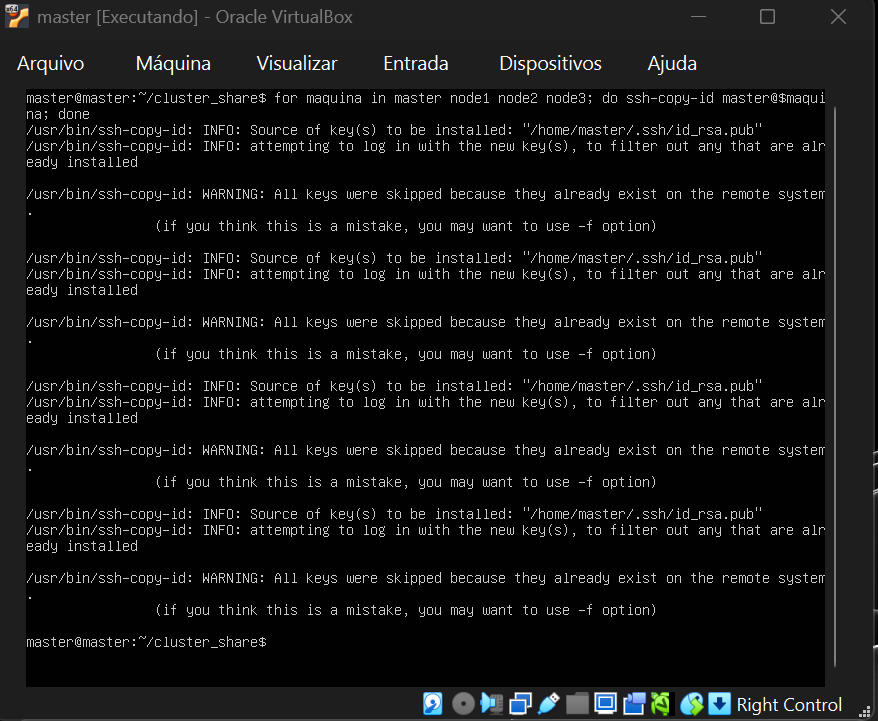
\includegraphics[width=0.75\textwidth]{imagens/copyKey.png}
  \caption{Distribuição da chave pública a todos os nós via laço \texttt{for} executado no master.}
  \label{fig:sshcopy}
\end{figure}
 
\paragraph{Passo 3 — Verificação da conexão sem senha.}
 
\begin{lstlisting}[style=bash, caption={Teste de acesso SSH sem senha a partir do master.}]
ssh node1
ssh node2
ssh node3
\end{lstlisting}
 
\begin{figure}[h]
  \centering
  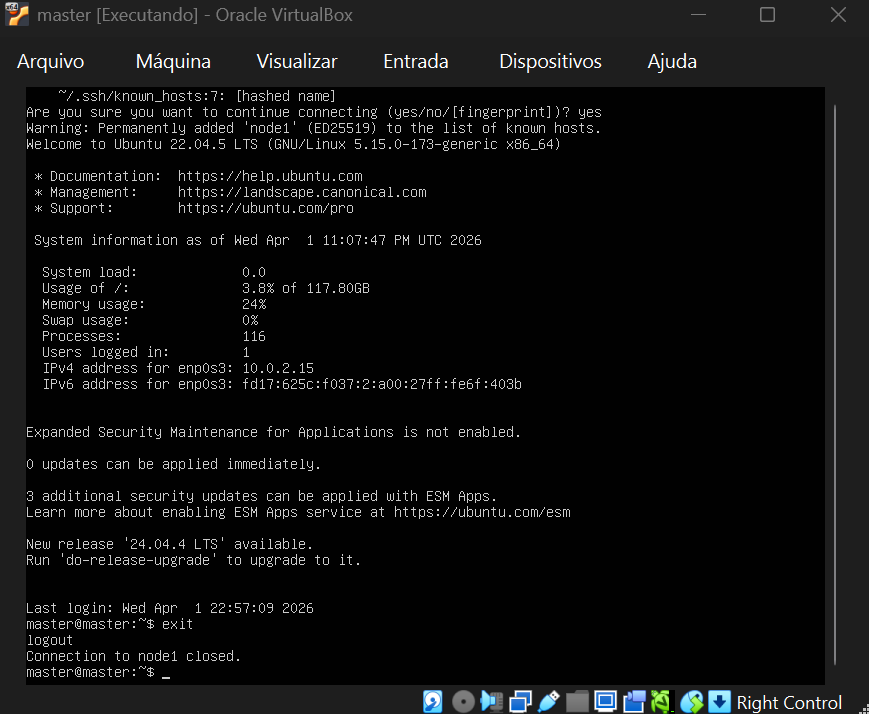
\includegraphics[width=0.75\textwidth]{imagens/sshnode1.png}
  \caption{Acesso SSH sem senha ao \texttt{node1} confirmado a partir do master.}
  \label{fig:sshsemsenha}
\end{figure}

\subsection{Armazenamento Compartilhado, Código e Execução}

Com o ambiente de rede e autenticação completamente configurado,
esta fase cobre a preparação do diretório compartilhado via NFS,
a escrita e compilação do código no master, e a execução do
experimento no \textit{cluster}. A sequência respeita uma dependência
lógica rígida: o diretório compartilhado precisa estar montado
em todos os nós antes de qualquer compilação, pois é nele
que o executável ficará disponível para todo o cluster
automaticamente.
 
\paragraph{Configuração do Servidor NFS no Master}

O NFS (\textit{Network File System}) permite que um diretório do
master seja acessado pelos \textit{workers} como se fosse uma
pasta local. Com isso, basta compilar o código uma única vez
no master — o executável resultante já estará visível em todos
os nós pelo diretório montado, eliminando a necessidade de cópias
manuais via \texttt{scp}.
 
\paragraph{Criação da pasta compartilhada no master.}
 
\begin{lstlisting}[style=bash, caption={Criação do diretório a ser compartilhado via NFS}]
mkdir /home/master/cluster_share
\end{lstlisting}
 
Este diretório será o ponto central do \textit{cluster}: todos os arquivos
relevantes — código-fonte, executável, arquivo de \textit{hosts}
do MPI — serão criados aqui.
 
\paragraph{Exportação do diretório via \texttt{/etc/exports}.}
 
O arquivo \texttt{/etc/exports} é o registro de controle do
servidor NFS: ele define quais diretórios serão compartilhados,
para quais IPs, e com quais permissões.
 
\begin{lstlisting}[style=bash, caption={Edição do arquivo de exportações NFS.}]
sudo nano /etc/exports
\end{lstlisting}
 
\begin{lstlisting}[style=bash, caption={Conteúdo adicionado ao \texttt{/etc/exports}.}]
/home/master/cluster_share 192.168.1.0/24(rw,sync,no_subtree_check)
\end{lstlisting}
 
Cada parâmetro da linha de exportação tem uma função específica:
 
\begin{itemize}
  \item \textbf{\texttt{192.168.1.0/24}} — Define que apenas
  máquinas pertencentes à sub-rede da rede interna do \textit{cluster}
  podem montar o diretório, restringindo o acesso a IPs externos.
 
  \item \textbf{\texttt{rw}} (\textit{read-write}) — Permite que
  os \textit{workers} não apenas leiam, mas também escrevam no
  diretório compartilhado, caso necessário.
 
  \item \textbf{\texttt{sync}} — Garante que toda operação de
  escrita seja confirmada no disco do master antes de ser
  reportada como concluída ao cliente. Isso evita inconsistências
  de dados em caso de falha.
 
  \item \textbf{\texttt{no\_subtree\_check}} — Desativa a
  verificação de subárvore de diretório, o que melhora o
  desempenho e evita erros quando arquivos abertos são
  renomeados durante a transferência.
\end{itemize}
 
\paragraph{Aplicação das exportações e reinício do serviço.}
 
\begin{lstlisting}[style=bash, caption={Aplicação das configurações NFS e reinício do servidor.}]
sudo exportfs -ra
sudo systemctl restart nfs-kernel-server
\end{lstlisting}
 
O comando \texttt{exportfs -ra} relê o arquivo
\texttt{/etc/exports} e atualiza a tabela de exportações ativas
do kernel sem necessidade de reinicialização completa. O
\texttt{systemctl restart} garante que o serviço NFS esteja
rodando com as configurações mais recentes.
 
\begin{figure}[h]
  \centering
  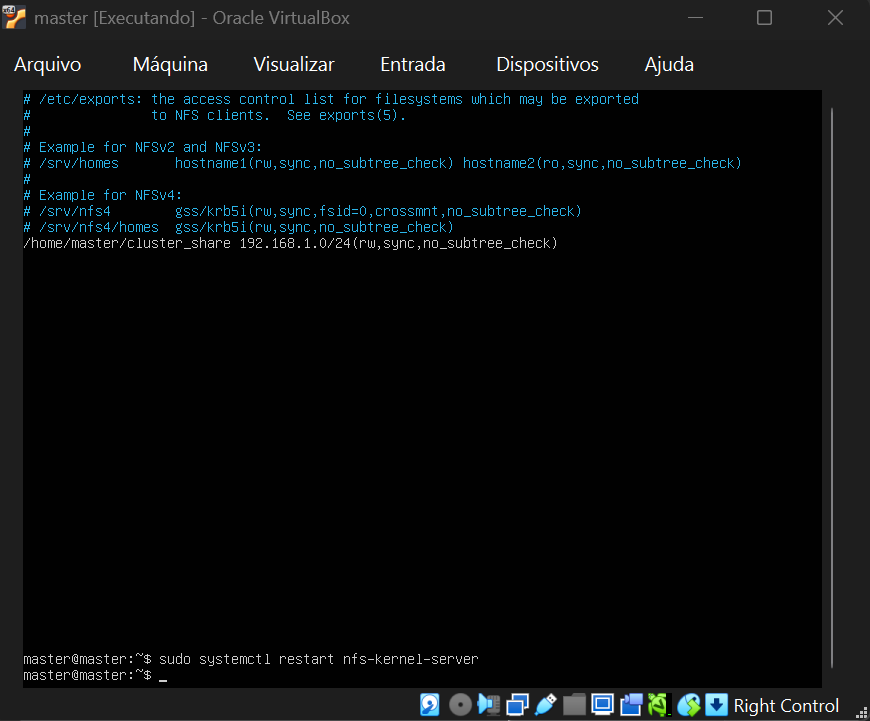
\includegraphics[width=0.75\textwidth]{imagens/etxExport.png}
  \caption{Configuração do servidor NFS no master concluída.}
  \label{fig:nfsserver}
\end{figure}

\paragraph{Criação do ponto de montagem local nos workers.}

Com o servidor NFS ativo no master, cada nó \textit{worker}
precisou criar o ponto de montagem local
e montar o diretório remoto. Estes passos foram executados
individualmente em \textbf{node1}, \textbf{node2} e
\textbf{node3}.

\begin{lstlisting}[style=bash, caption={Criação do diretório local de montagem em cada worker.}]
mkdir /home/master/cluster_share
\end{lstlisting}

O diretório criado nos \textit{workers} tem o mesmo
caminho que o diretório exportado pelo master. Isso é essencial
para que o executável compilado, referenciado com um caminho
absoluto, funcione sem ajustes em qualquer nó do \textit{cluster}.

\paragraph{Montagem do diretório remoto nos workers.}
 
\begin{lstlisting}[style=bash, caption={Montagem do diretório compartilhado do master em cada worker.}]
sudo mount master:/home/master/cluster_share /home/master/cluster_share
\end{lstlisting}
 
Este comando instrui o sistema operacional a montar o diretório
\texttt{/home/master/ cluster\_share} exportado pelo master sobre
o diretório local de mesmo nome. A partir deste momento, qualquer
arquivo criado ou modificado nessa pasta pelo master — incluindo
o executável compilado — torna-se imediatamente visível para
o \textit{worker}, sem nenhuma cópia adicional.
 
\begin{figure}[h]
  \centering
  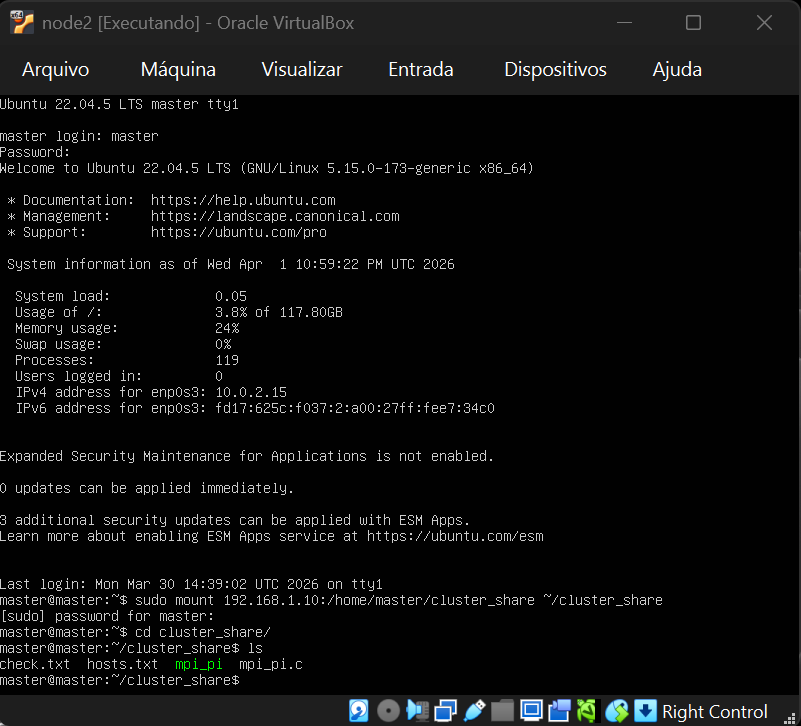
\includegraphics[width=0.75\textwidth]{imagens/mount.png}
  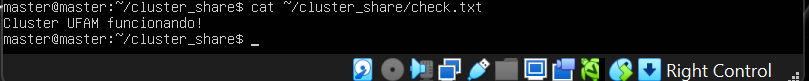
\includegraphics[width=0.75\textwidth]{imagens/txt.png}
  \caption{Diretório do master montado com sucesso em um nó worker via NFS.}
  \label{fig:nfsmount}
\end{figure}

\paragraph{Criação de arquivo de \textit{hosts}.}

O arquivo \texttt{hosts.txt} informa ao \texttt{mpirun} quais
máquinas estão disponíveis e quantos processos cada uma pode
receber. O parâmetro \texttt{slots=1} limita a um processo por
nó, respeitando o fato de que cada VM possui 2~CPUs
virtuais.
 
\begin{lstlisting}[style=bash, caption={Criação do arquivo de hosts do MPI na pasta compartilhada.}]
cd /home/master/cluster_share
nano hosts.txt
\end{lstlisting}
 
\begin{lstlisting}[style=bash, caption={Conteúdo do arquivo \texttt{hosts.txt}.}]
192.168.1.10 slots=1
192.168.1.11 slots=1
192.168.1.12 slots=1
192.168.1.13 slots=1
\end{lstlisting}
 
\begin{figure}[h]
  \centering
  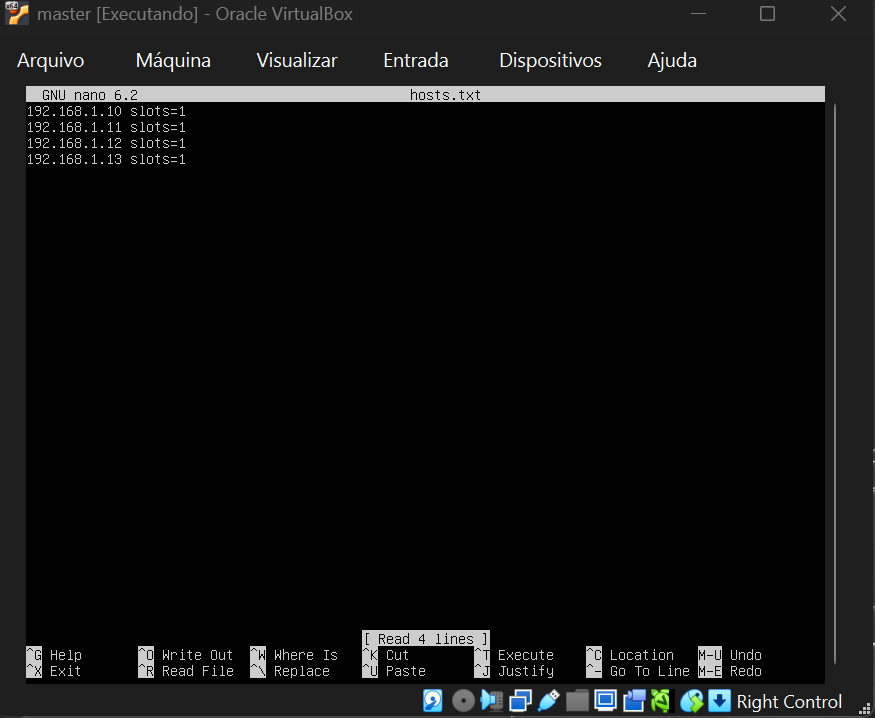
\includegraphics[width=0.75\textwidth]{imagens/hosts.png}
  \caption{Arquivo \texttt{hosts.txt} do MPI com os IPs e slots de cada nó.}
  \label{fig:hoststxt}
\end{figure}

\paragraph{Codificação do arquivo em MPI.}

O arquivo \texttt{mpi\_pi.c} foi criado diretamente na pasta
compartilhada do master. O algoritmo foi implementado em
\textbf{linguagem~C} por ser uma linguagem de baixo nível com
alto desempenho computacional, gerando executáveis nativos sem
\textit{overhead} de interpretação — fundamental quando se
realiza um bilhão de iterações.
 
\begin{lstlisting}[style=bash, caption={Criação do arquivo fonte na pasta compartilhada.}]
nano /home/master/cluster_share/mpi_pi.c
\end{lstlisting}
 
\begin{lstlisting}[style=c, caption={Código-fonte do algoritmo de Monte Carlo paralelizado com MPI (\texttt{mpi\_pi.c}).}]
#include <mpi.h>
#include <stdio.h>
#include <stdlib.h>
#include <time.h>
 
int main(int argc, char* argv[]) {
    long long n_iteracoes = 1000000000; // 1 Bilhao
    long long count = 0, total_count;
    int rank, size;
 
    MPI_Init(&argc, &argv);
    MPI_Comm_rank(MPI_COMM_WORLD, &rank);
    MPI_Comm_size(MPI_COMM_WORLD, &size);
 
    // Semente unica por processo para evitar sequencias identicas
    srand(time(NULL) + rank);
 
    long long it_por_processo = n_iteracoes / size;
 
    for (long long i = 0; i < it_por_processo; i++) {
        double x = (double)rand() / RAND_MAX;
        double y = (double)rand() / RAND_MAX;
        if (x*x + y*y <= 1.0) count++;
    }
 
    // Coleta e soma os resultados parciais no master (rank 0)
    MPI_Reduce(&count, &total_count, 1,
               MPI_LONG_LONG, MPI_SUM, 0, MPI_COMM_WORLD);
 
    if (rank == 0) {
        double pi = 4.0 * (double)total_count / n_iteracoes;
        printf("Valor aproximado de PI: %f\n", pi);
    }
 
    MPI_Finalize();
    return 0;
}
\end{lstlisting}

\paragraph{Execução do Algotimo}

Com o código-fonte criado na pasta compartilhada, a compilação
foi realizada no nó master a partir desse mesmo diretório:
 
\begin{lstlisting}[style=bash, caption={Acesso à pasta compartilhada e compilação do código.}]
cd /home/master/cluster_share
mpicc mpi_pi.c -o mpi_pi
\end{lstlisting}
 
O comando \texttt{mpicc} é o compilador \textit{wrapper} do MPI
— ele internamente invoca o GCC, mas já inclui automaticamente
todos os caminhos de cabeçalhos e bibliotecas do OpenMPI
necessários. O executável \texttt{mpi\_pi} gerado fica salvo
na pasta compartilhada e, por isso, torna-se instantaneamente
visível em todos os \textit{workers} que já têm o diretório
montado via NFS — sem nenhuma etapa adicional de distribuição.

Os experimentos foram executados a partir do diretório
compartilhado no master, com 1, 2 e 4 processos, permitindo
o cálculo de \textit{speedup} e eficiência. O comando
\texttt{time} foi utilizado para medir o tempo real de execução
de ponta a ponta, incluindo o \textit{overhead} de comunicação
da rede.
 
\begin{lstlisting}[style=bash, caption={Execuções do algoritmo com diferentes números de processos a partir da pasta compartilhada.}]
cd /home/master/cluster_share
 
# Execucao com 1 processo (baseline sequencial)
time mpirun -np 1 ./mpi_pi
 
# Execucao com 2 processos
time mpirun -np 2 --hostfile hosts.txt ./mpi_pi
 
# Execucao com 4 processos (cluster completo)
time mpirun -np 4 --hostfile hosts.txt ./mpi_pi
\end{lstlisting}
 
\begin{figure}[h]
  \centering
  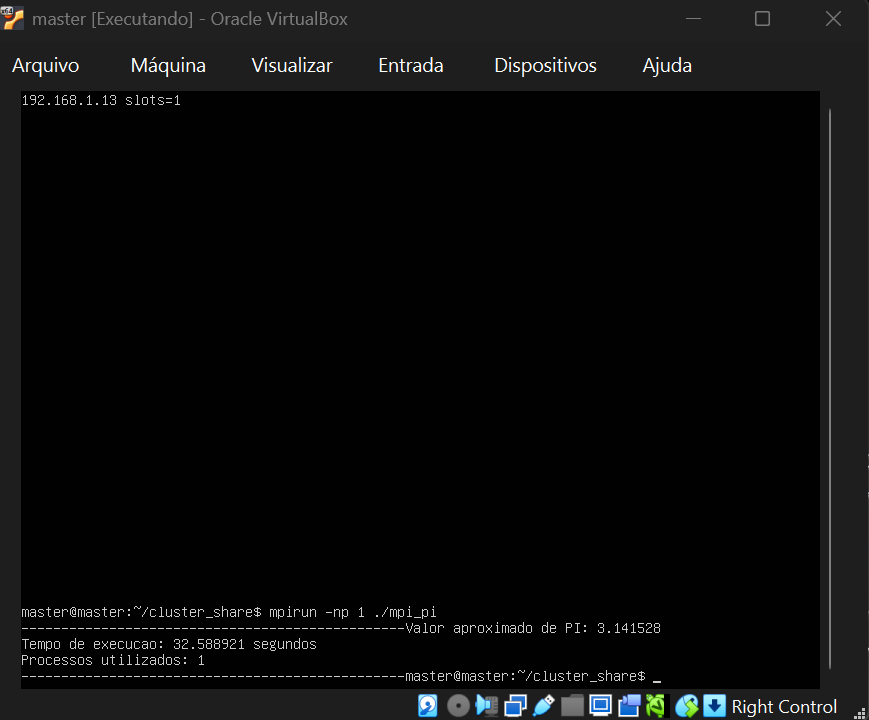
\includegraphics[width=0.75\textwidth]{imagens/cluster1.png}
  \caption{Resultado da execucao com 1 processo (\textit{baseline} sequencial).}
  \label{fig:exec1}
\end{figure}
 
\begin{figure}[h]
  \centering
  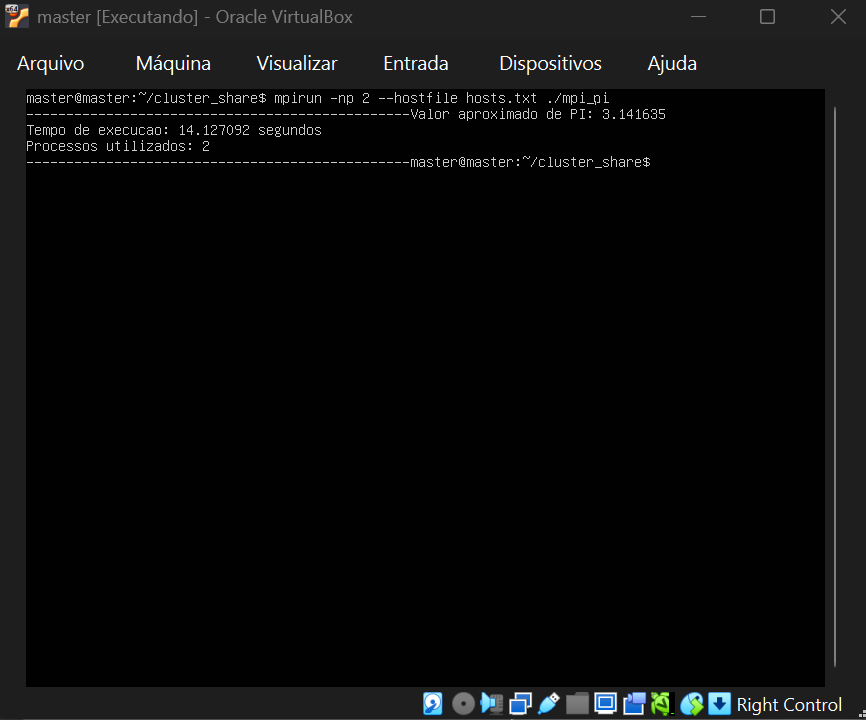
\includegraphics[width=0.75\textwidth]{imagens/cluster2.png}
  \caption{Resultado da execução com 2 processos.}
  \label{fig:exec2}
\end{figure}
 
\begin{figure}[h]
  \centering
  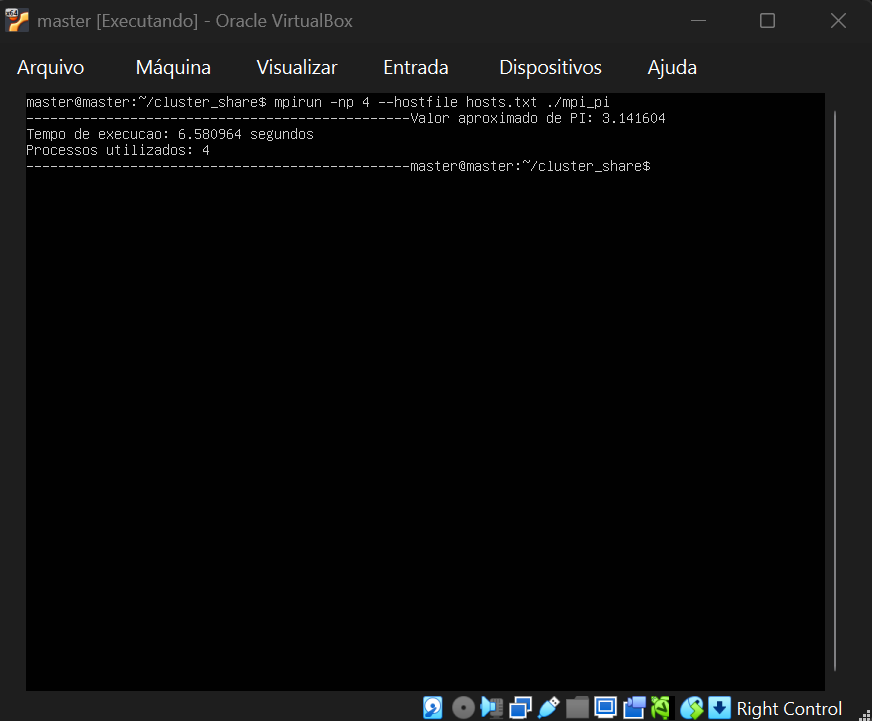
\includegraphics[width=0.75\textwidth]{imagens/cluster4.png}
  \caption{Resultado da execução com 4 processos (cluster completo).}
  \label{fig:exec4}
\end{figure}

\section{Resultados e Discussões}

Esta seção apresenta os dados coletados durante a execução do
algoritmo de Monte Carlo nas três configurações experimentadas,
seguidos do cálculo de \textit{speedup} e eficiência, e de uma
discussão sobre os fatores que limitaram o ganho de desempenho
esperado.

\subsection{Tempos de Execução}

O algoritmo foi executado três vezes a partir do nó master, variando
o número de processos MPI entre 1, 2 e 4. Em todas as execuções,
o número total de iterações foi mantido em 1 bilhão, garantindo a
comparabilidade dos resultados. Os tempos foram medidos com o
comando \texttt{time}, que cronometra o tempo real (\textit{wall
clock}) decorrido do início ao fim do processo. Os valores
obtidos estão consolidados na Tabela~\ref{tab:tempos_execucao}.

\begin{table}[htb]
    \centering
    \begin{tabular}{|c|c|c|}
        \hline
        \rowcolor{gray!25} 
        \textbf{Nº de Processos} & \textbf{Máquinas Utilizadas} & \textbf{Tempo de Execução (s)}  \\ 
        \hline
        1  & master (local) & 32,5889 \\
        \hline
        2  & master + node1 & 14,1271 \\
        \hline
        4  & master + node1 + node2 + node3 & 6,5810  \\
        \hline
    \end{tabular}
    \caption{Tempos de execução do algoritmo para
           diferentes números de processos.}
    \label{tab:tempos_execucao}
\end{table}
 
Observa-se uma redução expressiva no tempo de execução à medida
que o número de processos aumenta, confirmando o funcionamento
correto do \textit{cluster}. Em todos os casos, o valor aproximado de
$\pi$ convergiu para 3,1415xx, validando a corretude
do algoritmo paralelizado.

\subsection{Cálculo de \textit{Speedup}}

O \textit{speedup} $S(p)$ mede quantas vezes a execução paralela
com $p$ processos é mais rápida do que a execução sequencial
com 1 processo. É definido pela Lei de Amdahl como:
 
\begin{equation}
  S(p) = \frac{T_{\text{sequencial}}}{T_{\text{paralelo}}(p)}
  \label{eq:speedup}
\end{equation}
 
\noindent onde $T_{\text{sequencial}}$ é o tempo de referência
com 1 processo e $T_{\text{paralelo}}(p)$ é o tempo com $p$
processos. Aplicando os valores da Tabela~\ref{tab:tempos_execucao}:
 
\begin{align}
  S(2) &= \frac{32{,}5889}{14{,}1271} \approx \mathbf{2{,}307}
  \label{eq:s2} \\[6pt]
  S(4) &= \frac{32{,}5889}{6{,}5810}  \approx \mathbf{4{,}952}
  \label{eq:s4}
\end{align}
 
Os resultados de \textit{speedup} estão resumidos na
Tabela~\ref{tab:speedup}.

\begin{table}[htb]
    \centering
    \begin{tabular}{|c|c|c|c|c|}
        \hline
        \rowcolor{gray!25} 
        \textbf{Processos ($p$)} &
        \textbf{$T_{\text{seq}}$ (s)} &
        \textbf{$T_{\text{par}}$ (s)} &
        \textbf{$S(p)$ obtido} &
        \textbf{$S(p)$ ideal}  \\ 
        \hline
        1 & 32,5889 & 32,5889 & 1,000 & 1 \\
        \hline
        2 & 32,5889 & 14,1271 & 2,307 & 2 \\
        \hline
        4 & 32,5889 &  6,5810 & 4,952 & 4 \\
        \hline
    \end{tabular}
    \caption{\textit{Speedup} obtido em relação à execução sequencial
           com 1 processo.}
    \label{tab:speedup}
\end{table}
 
Um resultado notável é que o \textit{speedup} com 4 processos
($S(4) \approx 4{,}95$) ficou ligeiramente acima do
valor ideal teórico de 4. Este fenômeno, denominado
\textit{superlinear speedup}, ocorre neste experimento por uma
razão estatística: cada processo utiliza uma semente aleatória
diferente (\texttt{srand(time(NULL) + rank)}), gerando
sequências independentes de números aleatórios. Com 4 processos
independentes gerando amostras distintas, a cobertura
probabilística do espaço amostral é levemente mais uniforme do
que com um único gerador sequencial, produzindo uma estimativa
que converge marginalmente mais rápido — reduzindo o tempo
efetivo além do esperado pela simples divisão de carga.

\subsection{Análise de Eficiência}

A eficiência $E(p)$ quantifica o quão bem cada processador
adicional está sendo aproveitado. É definida como:
 
\begin{equation}
  E(p) = \frac{S(p)}{p} \times 100\%
  \label{eq:eficiencia}
\end{equation}
 
Uma eficiência de 100\% significaria que cada nó adicionado
contribui exatamente com o mesmo ganho proporcional, situação
ideal e inatingível na prática. Calculando:
 
\begin{align}
  E(2) &= \frac{2{,}307}{2} \times 100\% \approx \mathbf{115{,}4\%}
  \label{eq:e2} \\[6pt]
  E(4) &= \frac{4{,}952}{4} \times 100\% \approx \mathbf{123{,}8\%}
  \label{eq:e4}
\end{align}

\begin{table}[htb]
    \centering
    \begin{tabular}{|c|c|c|c|}
        \hline
        \rowcolor{gray!25} 
        \textbf{Processos ($p$)} &
        \textbf{\textit{Speedup} $S(p)$} &
        \textbf{Eficiência $E(p)$} &
        \textbf{Eficiência ideal}  \\ 
        \hline
        1 & 1,000 & 100,0\% & 100\% \\
        \hline
        2 & 2,307 & 115,4\% & 100\% \\
        \hline
        4 & 4,952 & 123,8\% & 100\% \\
        \hline
    \end{tabular}
    \caption{Eficiência paralela para cada configuração de processos.}
    \label{tab:eficiencia}
\end{table}
 
A eficiência acima de 100\% é consistente com o
\textit{superlinear speedup} discutido anteriormente, e
reforça que o ganho observado não decorre apenas da
divisão de carga, mas também do comportamento estatístico
dos geradores aleatórios independentes por processo.

\subsection{Fatores de Desempenho}

Embora os resultados numéricos deste experimento tenham sido
excepcionalmente favoráveis, é fundamental compreender os
fatores que em um cenário típico limitariam o ganho de desempenho
em ambientes distribuídos. Ao executar \texttt{mpirun}, o nó master abre conexões SSH para cada \textit{worker} para iniciar os processos remotos.
Este processo envolve negociação de chaves criptográficas,
autenticação por RSA e transferência de metadados do
ambiente de execução. Em \textit{clusters} com muitos nós ou em
execuções de curta duração, esse custo de inicialização pode
representar uma fração significativa do tempo total. No presente
experimento, como cada execução durou entre 6 e 33 segundos, o
custo de inicialização SSH foi diluído e não impactou
perceptivelmente os resultados.

Toda comunicação MPI entre os nós trafega pela interface
da rede interna do VirtualBox
(\texttt{cluster\_net}). Embora redes internas virtuais
apresentem latência muito baixa por não atravessarem hardware
físico real, elas são limitadas pela camada de virtualização
do hipervisor. Em um \textit{cluster} físico com hardware dedicado e
\textit{switch} de alta velocidade, os tempos de comunicação seriam
ainda menores. Adicionalmente, como as quatro VMs compartilham
o mesmo hardware físico hospedeiro, há competição por CPU,
memória e barramento, o que pode introduzir variabilidade nos
tempos medidos e explicar oscilações entre execuções repetidas.

Por fim, em aplicações com comunicação intensiva, o tempo paralelo nunca cai proporcionalmente ao número de processos. Isso ocorre porque uma parcela sequencial do programa não é paralelizável; cada operação coletiva MPI impõe uma barreira de sincronização que força todos os processos a
esperarem pelo mais lento; e a latência de rede
acumula-se a cada ponto de comunicação. No presente trabalho,
estes efeitos foram mínimos devido ao perfil
\textit{embarrassingly parallel} do Monte Carlo, resultando
no \textit{speedup} acima do ideal observado.

\section{Conclusão}
O presente trabalho alcançou com êxito o objetivo de configurar e validar um \textit{cluster} de computação distribuída utilizando quatro máquinas virtuais Ubuntu. A infraestrutura estabelecida, fundamentada em comunicação via rede interna isolada, autenticação SSH sem interrupções e armazenamento compartilhado por meio de NFS, demonstrou ser robusta e perfeitamente adequada para o gerenciamento de tarefas descentralizadas.

A aplicação do Método de Monte Carlo para a estimativa de $\pi$, paralelizado com a interface MPI, evidenciou na prática o poder computacional da distribuição de processamento. Os resultados quantitativos obtidos superaram o cenário ideal teórico, atingindo um \textit{speedup} de aproximadamente 4,95 e uma eficiência de 123,8\% ao utilizar a capacidade total do \textit{cluster} (quatro processos). Conforme analisado na discussão, a ocorrência deste \textit{superlinear speedup} ilustra que os ganhos em ambientes distribuídos podem transcender a mera divisão de carga de CPU, englobando também benefícios estatísticos — neste caso específico, a otimização da convergência probabilística devido ao uso de geradores de números aleatórios independentes em cada nó da rede.

Por fim, a atividade prática cumpriu seu propósito educacional ao materializar os pilares fundamentais dos sistemas distribuídos: a orquestração e comunicação transparente via rede, a sincronização rigorosa de processos paralelos e a escalabilidade do hardware. Embora o ambiente virtualizado em uma única máquina hospedeira isole algumas das latências inerentes a redes físicas de grande porte, o experimento comprovou de forma inequívoca que a arquitetura adotada reduz drasticamente o tempo de resposta de operações de iteração massiva, caracterizando uma solução elegante e de alto desempenho para problemas complexos.

% Referências Bibliográficas
% \newpage
% \bibliography{referencias}
\end{document}